\section{Fiducial System Modifications}
\label{section:fiducial_system_modifications}

After the initial proof of concept attempt at fiducial-based landing with a gimbal-mounted camera (shown in Section~\ref{section:initial_hexacopters}),
we have decided to make some modifications to the tested fiducial systems to make a success more likely.
To restate, the goal is to successfully execute precision landings using a fiducial marker to designate a landing site,
and the key difference between this work and previous work is the gimbal-mounted camera for marker tracking.
Most previous projects use a fixed, downward facing camera and have reported loss of sight of the landing pad due to
wind and thrust vectoring by the drone.
Marker tracking makes the detection of the landing pad more robust to the drone's movements,
but also complicates the pose estimation.
Since the orientation of the camera cannot be assumed to be straight down,
we must transform the pose of the detected fiducial marker in order to generate a position target.
However, due to the planar pose estimation problem, the detected orientation is unreliable in monocular detection of planar fiducial markers,
as shown in Figure~\ref{figure:discontinuities}.
To mitigate the issue of orientation ambiguity, we have created 3 new variants of the April Tag and WhyCode fiducial systems,
and compared them to 2 default variants, as outlined below.
This is the content of a paper we have submitted to IROS 2022.

\subsection{Methods}

\begin{figure}
    \centering
    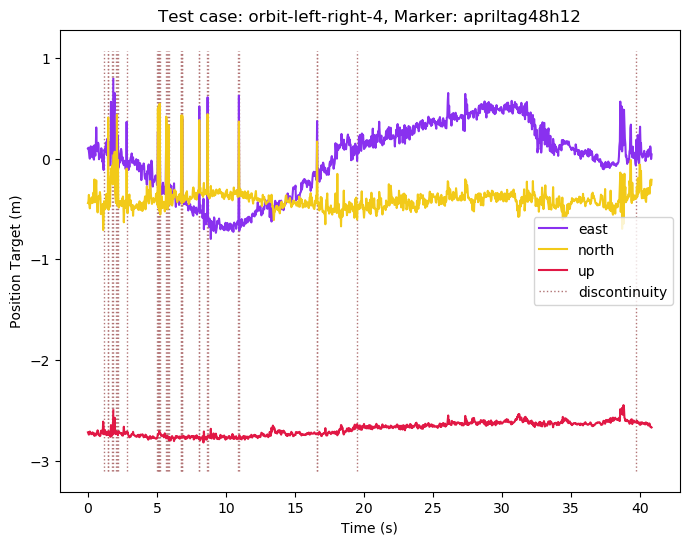
\includegraphics[width=0.5\textwidth]{orbit-left-right-4_apriltag48h12_position-target}
    \caption{Demonstration of discontinuities in position targets as a result of orientation ambiguity.}
    \label{figure:discontinuities}
\end{figure}

\subsubsection{WhyCode Orig: Tooth Arclength Sampling}
\label{section:whycode_orig}
We use a version of WhyCode created by Ulrich~\cite{ulrich} as a baseline for testing.
The method samples the ellipse that goes through the centers of the ``teeth'' forming the marker's ID
(i.e.~the yellow and green ellipses in Figure~\ref{figure:whycode_orig}),
to determine the marker's orientation.
Of the 2 possible candidate solutions that are implied by the detected semi-axes of the outer black ellipse, the detector chooses the one that has lower variance on the number of sample points per tooth.
This works because the candidate solutions predict this ellipse to be in slightly different places,
and the correct solution should predict the ellipse to be in its correct place,
minimizing the variance in the number of sample points that coincide with each tooth.
Conversely, the incorrect solution should predict the ellipse to be in the incorrect place,
such that the sampling ellipse does not line up well with the marker, and the variance is higher.
We use WhyCode markers with 8-bit IDs, so that there are several sample points and a meaningful variance.

\begin{figure}
    \centering
        \begin{subfigure}[b]{0.48\textwidth}
        \centering
        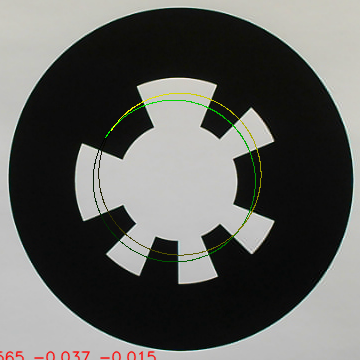
\includegraphics[width=\textwidth]{images/whycode_orig_both_solutions_cropped}
        \caption{WhyCode Orig method.}
        \label{figure:whycode_orig}
    \end{subfigure}
    \begin{subfigure}[b]{0.48\textwidth}
        \centering
        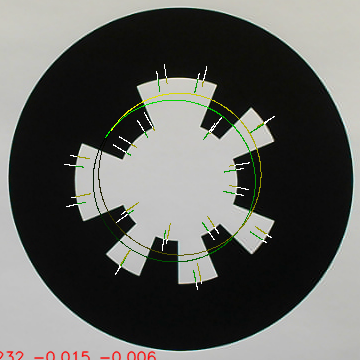
\includegraphics[width=\textwidth]{images/whycode_ellipse_both_solutions_cropped}
        \caption{WhyCode Ellipse method.}
        \label{figure:whycode_ellipse}
    \end{subfigure}
\end{figure}

\subsubsection{WhyCode Ellipse: Radial Tooth Sampling}
The first method that we have created for reducing orientation ambiguity is the \texttt{ellipse\_sampling} branch of~\cite{uzgit_whycon}.
The method determines the marker ID and the two candidate solutions for the orientation as in WhyCode Orig,
after which it identifies the lines that goes from the center of the white region through the center of each tooth.
It then samples the input image on these lines,
as illustrated by the radial sample lines in Figure~\ref{figure:whycode_ellipse}.
It expects a white-to-black transition at the predicted edge of each tooth, and the sampling line is centered on this edge.
The true edge is determined during sampling, and its value is recorded as a percentage of the length of the line segment,
oriented such that 0 corresponds to the centermost end of the line segment, and 1 corresponds to its outermost end.
The detector chooses the solution that minimizes the variance of the location of the true edge over the sample lines.

\subsubsection{WhyCode Multi: Planar Regression from Multiple Markers}
The second method that we have created for reducing orientation ambiguity (the \texttt{multi} branch of~\cite{uzgit_whycon})
works under the assumption that all markers are co-planar.
For each input image, the WhyCode algorithm identifies all markers and
then finds the normal vector to the plane implied by the markers' positions,
after which it can calculate the pitch and roll components of the bundle's orientation.
The position of the bundle is defined to be the mean of the positions of its constituent markers,
and its yaw is that of any constituent markers, with the assumption they are all the same.
The detector then calculates all additional attributes for the bundle as if it were a marker.
This system is tested on an arrangement of 3 co-planar, 8-bit WhyCode markers.

\subsubsection{April Tag 48h12: Large, Embeddable April Tag Family}
April Tag provides a default family 48h12, shown in Figure~\ref{figure:apriltag48h12},
for which the 4 center squares are undefined,
20 squares provide a white border,
28 squares provide a black border,
and 48 squares provide data bits,
giving a total of 96 defined squares.
The undefined center provides a space to embed a smaller marker,
which is useful in the last stages of a drone landing scenario,
where the camera is too close to the landing pad to see the larger markers.
We test this family as a baseline for the performance of April Tag.

\subsubsection{April Tag 24h10: Small, Embeddable April Tag Family}
We have created an April Tag 24h10 family (shown in Figure~\ref{figure:apriltag24h10_example}) in response to our
We have created an April Tag 24h10 family (shown in Figure~\ref{figure:apriltag24h10_example}) in response to our
initial experiments, which showed that April Tag 48h12 has a slower detection rate than WhyCode on embedded hardware.
We maintain marker embeddability while decreasing the size of the marker definition,
by reducing the size of the undefined center to region to 1 square, and adjusting the surrounding regions accordingly:
8 squares for a white border, 16 squares for a black border, and 24 outer data squares.
This gives a total of 48 defined squares(compared to the 96 squares of April Tag 48h12).
We test April Tag 24h10 to see if it can offer an increase in detection rate with respect to April Tag 48h12.

\subsection{Performance}

\subsubsection{Discontinuity Rates:}
We have achieved a lower rate of discontinuities in our WhyCode Ellipse system than the WhyCode Orig system.
Figure~\ref{figure:discontinuity_rates} shows the discontinuity rates of each system,
and Figure~\ref{figure:detection_rates} shows the detection rates.
Formal statistical tests (included in the paper) rank the systems against one another.

\begin{figure}
    \centering
        \begin{subfigure}[b]{0.48\textwidth}
        \centering
        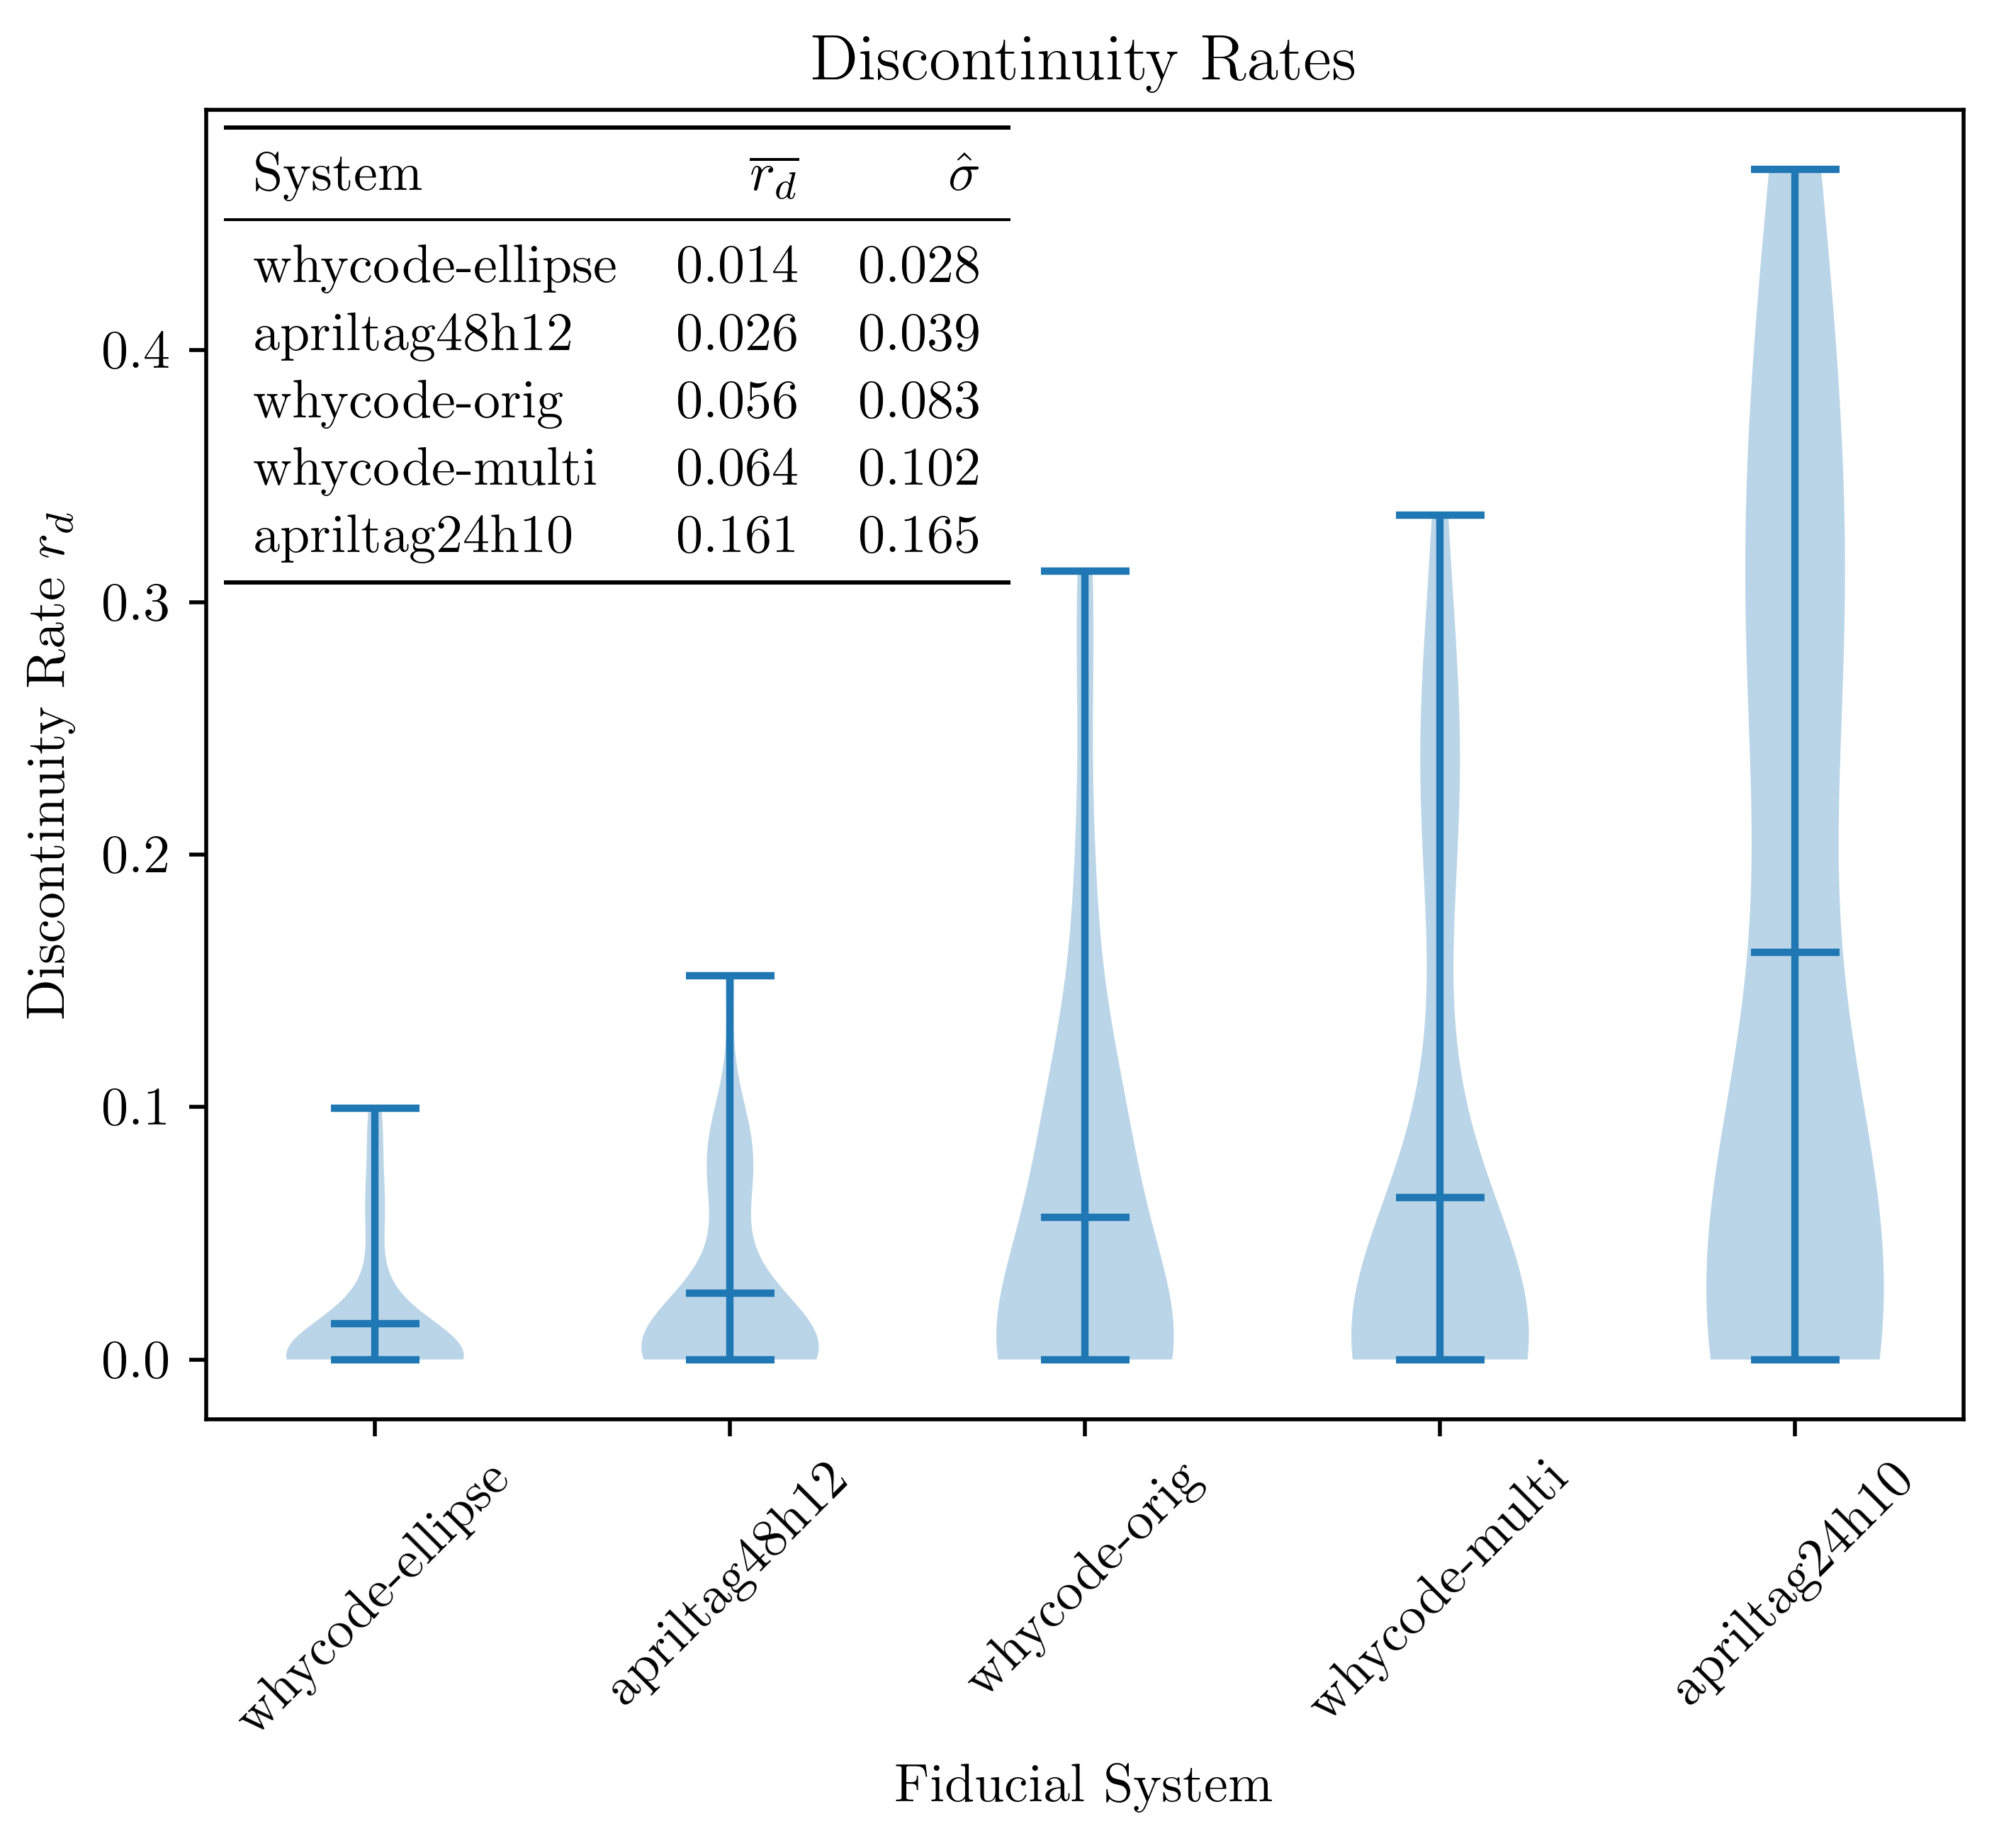
\includegraphics[width=\textwidth]{images/violin_plot_five_member}
        \caption{Discontinuity rates of the detected systems.}
        \label{figure:discontinuity_rates}
    \end{subfigure}
    \begin{subfigure}[b]{0.48\textwidth}
        \centering
        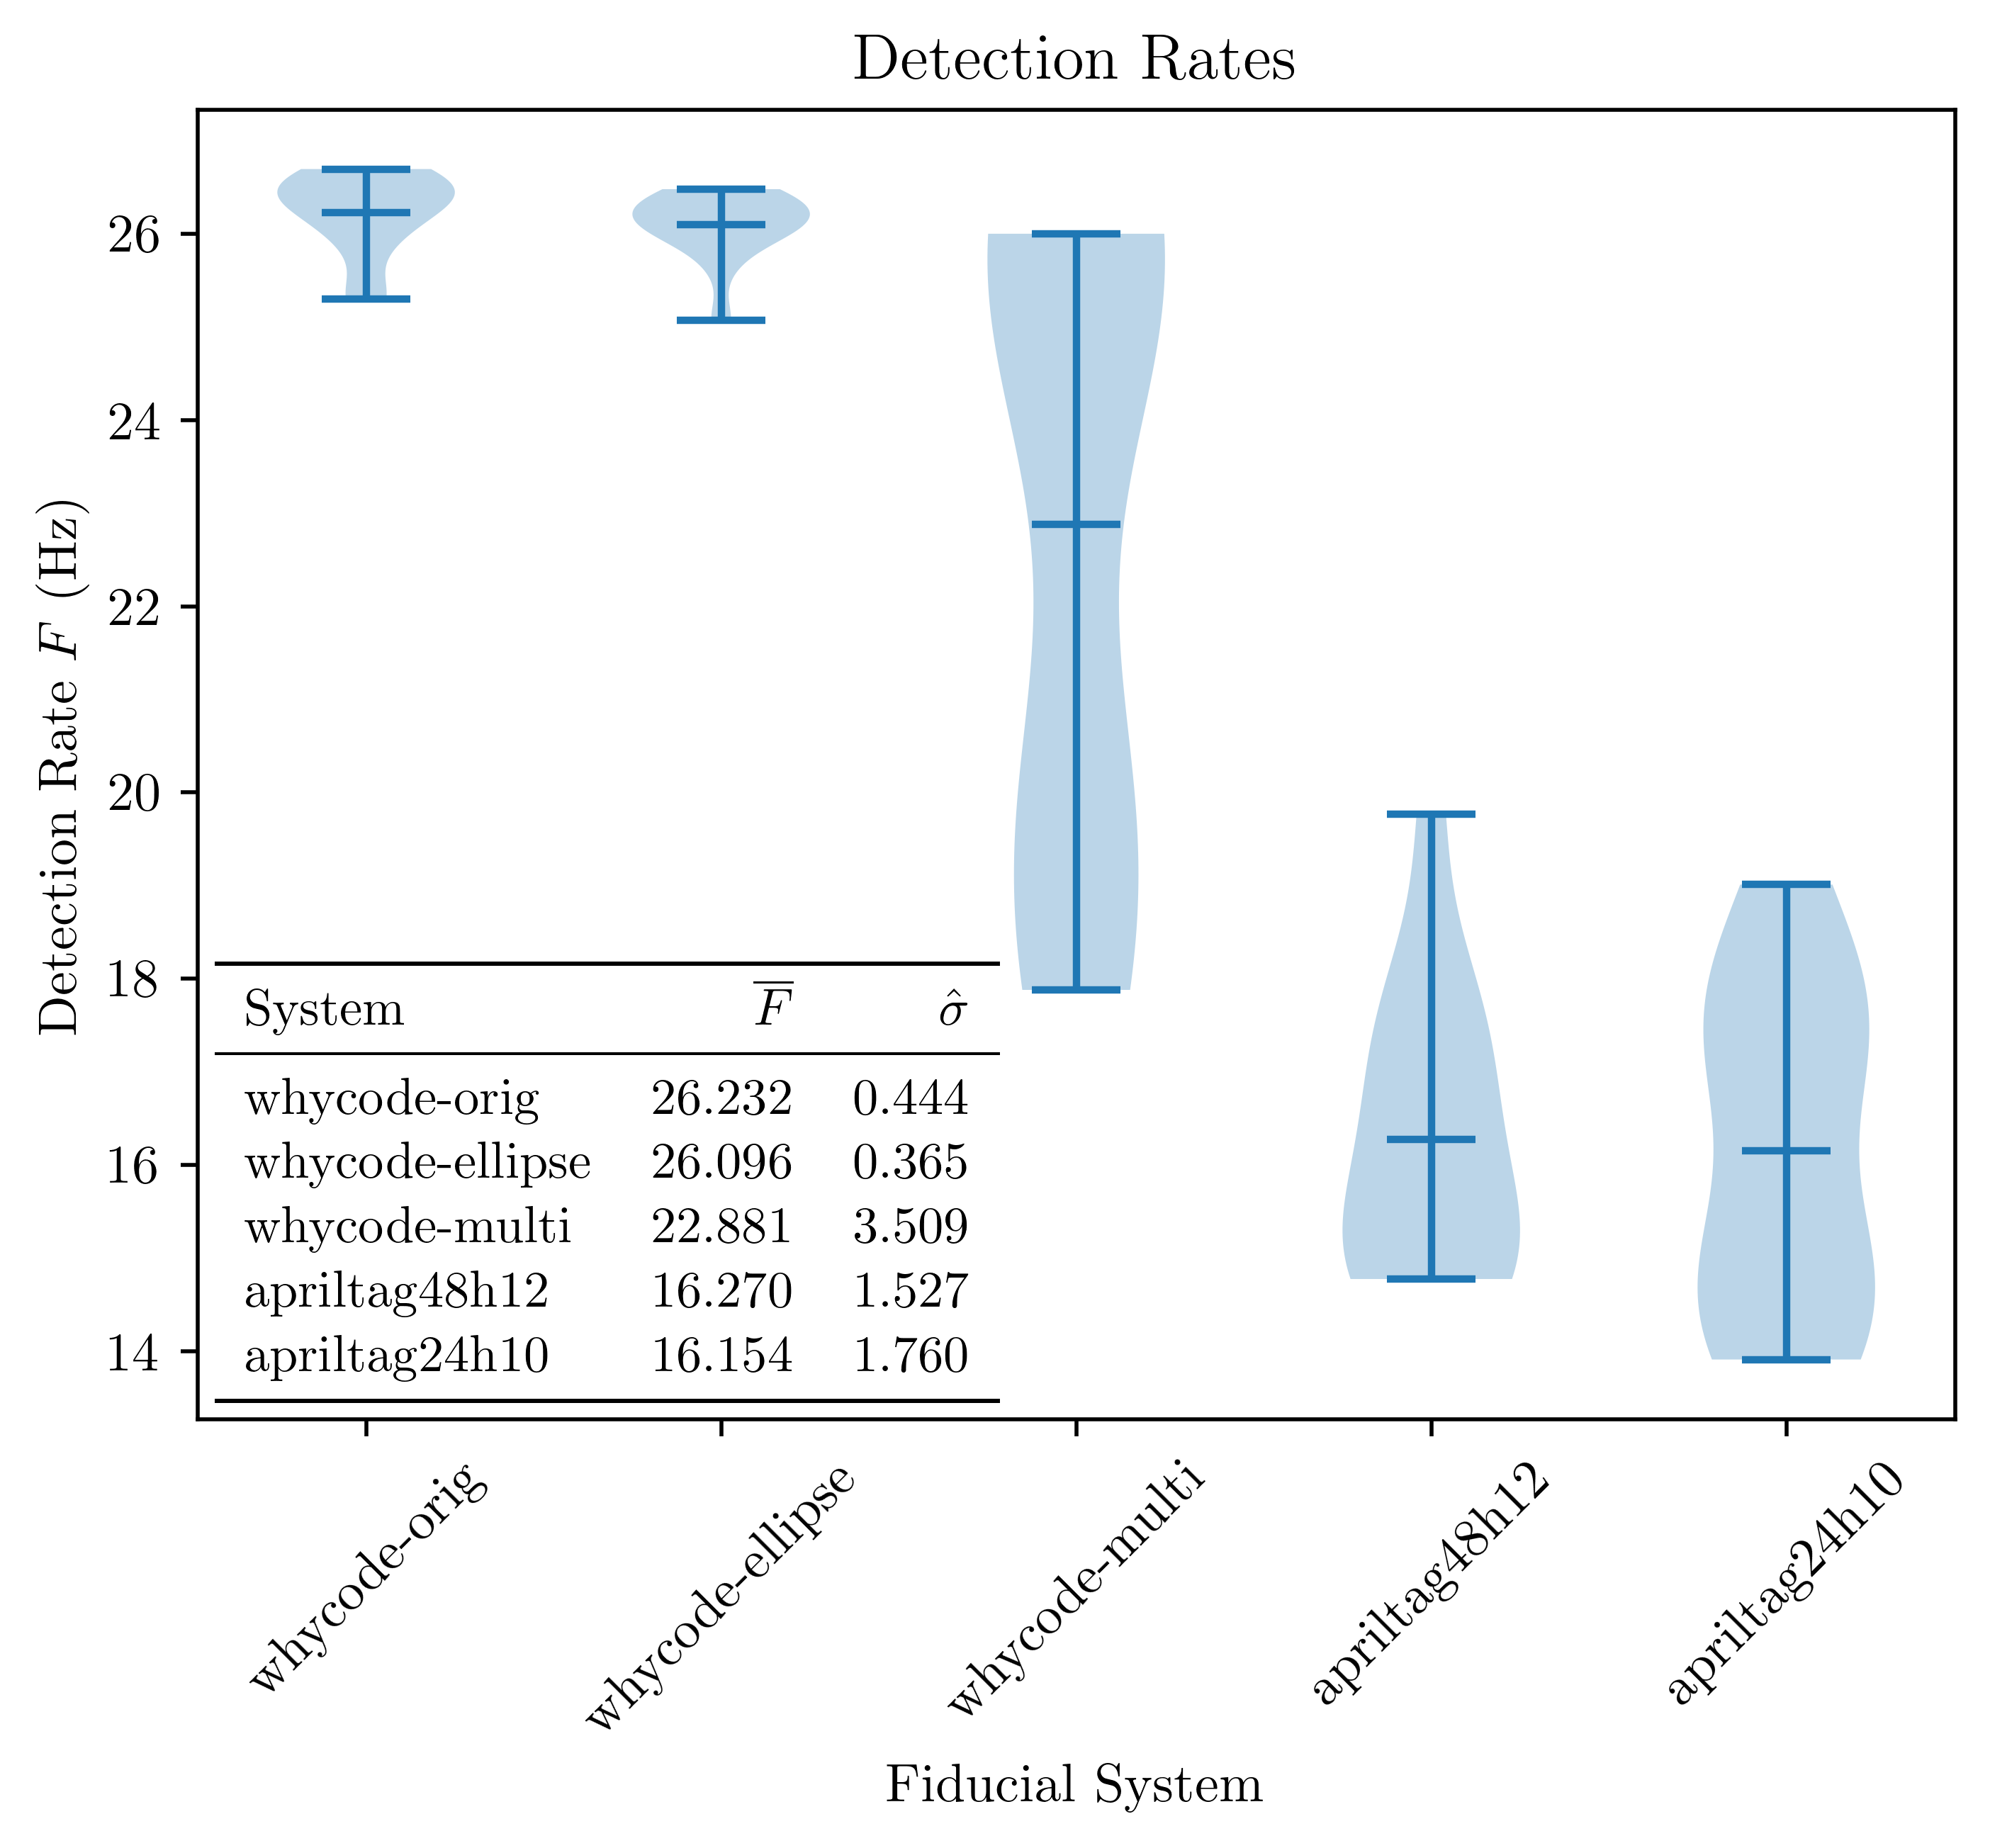
\includegraphics[width=\textwidth]{images/violin_plot_speed_five_member}
        \caption{Detection rates of the detected systems.}
        \label{figure:detection_rates}
    \end{subfigure}
\end{figure}